\documentclass[11pt]{article}
\usepackage[a4paper,margin=2.5cm]{geometry}
\usepackage[T1]{fontenc}
\usepackage[utf8]{inputenc}
\usepackage{amsmath,amssymb}
\usepackage{booktabs,array}
\usepackage{graphicx}
\usepackage{xcolor}
\usepackage{listings}
\usepackage[numbers,sort&compress]{natbib}
\usepackage[colorlinks=true,linkcolor=blue!50!black,citecolor=blue!50!black,urlcolor=blue!50!black]{hyperref}
\lstset{basicstyle=\ttfamily\small,columns=fullflexible,frame=single,framerule=0.3pt,
  rulecolor=\color{black!30},xleftmargin=4pt,xrightmargin=4pt}

\newcommand{\qZ}{qg_Z}

\title{Symmetry-filtered read-out on IBM quantum devices:\\
the qg filter on twenty device noise models through IBM Runtime}
\author{Vicente Humberto Monteverde\\
\small Universidad del Museo Social Argentino (UMSA), Argentina\\
\small ORCID 0000-0001-8884-4811}
\date{\small Draft of 13 October 2026}

\begin{document}
\sloppy
\maketitle

\begin{abstract}
Circuits built from gates that conserve the Hamming weight keep their state in one weight sector, so the
shots that left the sector can be discarded at read-out: the qg filter of the open-source library
qang~\cite{monteverde2026qang}, a form of symmetry verification~\cite{bonetmonroig2018,mcardle2019}. We
make it usable on IBM devices through IBM Runtime and Qiskit, and measure it on the noise models of twenty
IBM devices. The library adds a Qiskit transpiler pass that decides whether the filter applies, read-out
correction from each device's published per-qubit errors, qg read-outs of IBM Runtime Sampler and
Estimator results, zero-noise extrapolation by gate folding that stacks with the filter, a prediction of
the filter's kept fraction from the calibration, qubit selection with that prediction, a shot planner, and
the weight-conserving quantum neural network (QNN) of qang as one parameterized job and as a
qiskit-machine-learning \texttt{SamplerQNN}. Every prediction was committed before its run and is reported
as passed or failed. On ten five-qubit weight-1 circuits the filter lowers the error of the measured
$\qZ=\langle Z\rangle$ from 0.065--0.104 to 0.018--0.023 on three devices (0.013--0.022 with read-out correction), and filter plus zero-noise
extrapolation reaches 0.011--0.015. On seventeen further devices never used before, the filter cuts the
error 2.4--8.9$\times$ on every one (median 3.1$\times$ with read-out correction). Choosing the qubits by
the predicted kept fraction keeps 6--17 points more shots than Qiskit's default layout on chain circuits,
avoids a qubit published as reading 1 always, and the shot planner met a 0.02 target precision on three
devices. For classification the gain is small: the QNN recovers 5--6 of the 10 decisions noise costs it. Reading a
known five-component principal-component spectrum out of the data's density matrix in the weight-1 sector,
filter plus read-out correction lowers the error 4.6$\times$ (median over twenty-one devices) and orders the
spectrum correctly on 18 of 21 (13 raw). In Trotter simulation of the XY chain the filter halves the best
error and moves the optimal number of Trotter steps deeper (16 of 21 devices), and in a quantum walk it turns
a raw spreading indistinguishable from a classical random walk (exponent 0.87) into ballistic spreading
(1.84). With two or three interacting excitations (XXZ chain) the gain falls from 5.6$\times$ to
2.6$\times$: larger sectors let more of the noise through.
Two interoperability bugs were found, one in qiskit-machine-learning and one in the library. All results are
on device noise models; no hardware run is reported.
\end{abstract}

\noindent\textbf{Keywords:} quantum error mitigation; symmetry verification; post-selection; IBM Quantum;
quantum machine learning.

\section{Introduction}

When every gate of a circuit conserves the number of excitations (the Hamming weight of the computational
state), noise that changes that number moves shots out of the sector the circuit started in. Discarding
them is symmetry verification by post-selection~\cite{bonetmonroig2018,mcardle2019}. In qang it is the qg
filter, read in the unit $\qZ=\langle Z\rangle\in[-1,1]$~\cite{monteverde2026qang}; a companion note studies
it for quantum neural networks under relaxation~\cite{monteverde2026qml}.

This paper asks what the filter is worth on IBM devices and gives the tools to use it there: everything
runs through IBM Runtime~\cite{qiskitibmruntime} and Qiskit~\cite{javadiabhari2024qiskit}, here in local
testing mode on the device noise models (fake backends), unchanged on a device. Each experiment fixed its
circuits, settings and predictions in a commit before running; failures are reported as such. Sections
§137--§148 refer to the research notes of the repository, where every number below is reproduced by a
script in \texttt{examples/}.

\section{Methods}

\paragraph{Applicability.} \texttt{WeightPreservationCheck} is a Qiskit analysis pass. It marks a circuit as
weight-preserving when every gate conserves the excitation number (by name for gates such as RZ, CZ, SWAP or
XX+YY, otherwise from its matrix), and returns the initial weight prepared by leading X gates. It is run on
the logical circuit: after transpilation the native gates are not weight-preserving one by one.

\paragraph{Read-out.} For a circuit transpiled to a device, \texttt{ibm\_qg} reads the measured physical
qubits, takes their published asymmetric read-out errors $P(1|0)$, $P(0|1)$, and inverts the tensor product
of the per-qubit confusion matrices on the measured distribution~\cite{bravyi2021readout}. It returns
$\qZ$ per qubit raw, read-out corrected, filtered (weight-$w$ shots of the raw distribution) and filtered
after correction (the weight-$w$ part of the corrected quasi-distribution, renormalized). Qubits whose
confusion matrix cannot be inverted are left uncorrected and reported.

\paragraph{Kept fraction and qubit selection.} \texttt{predict\_kept\_fraction} multiplies the probability
that each calibrated channel leaves the weight unchanged: a single-qubit gate of error $e$ changes it with
probability $e$, a two-qubit gate with $5e/6$, relaxation over the busy time $t$ of a qubit with
$(1-e^{-t/T_1})\,w/n$, pure dephasing during the gates with $2z/3$, $z=(1-e^{-t/T_\phi})/2$, and read-out
with $\tfrac{w}{n}P(0|1)+(1-\tfrac{w}{n})P(1|0)$. Adding the shots that return to the sector as for a fully
mixed state gives \texttt{kept\_mixed\_floor}. \texttt{best\_chain} and \texttt{best\_layout} choose the
initial layout with the highest prediction; \texttt{best\_layout} scores the circuit as it will run, routing
included, and counts Qiskit's default layout among the candidates.

\paragraph{Zero-noise extrapolation.} IBM Runtime's own mitigation has no effect in local mode, so
\texttt{zne\_qg} folds every two-qubit gate ($G\to GG^\dagger G$, scale 3)~\cite{giurgicatiron2020}, runs
both scales and extrapolates linearly to zero~\cite{temme2017}. Folding keeps a weight-preserving circuit
weight-preserving, so it stacks with the filter.

\paragraph{Shot planning.} A filtered $\qZ$ read from $Nk$ kept shots has standard error
$\sqrt{(1-\qZ^2)/(Nk)}$. \texttt{plan\_shots} returns the $N$ that brings the worst qubit to a target error
with the predicted $k$, and the device time $N$(circuit duration + repetition delay).

\paragraph{QNN.} The weight-1 QNN of qang~\cite{monteverde2026qml} (an amplitude loader and three layers of
Hamming-weight-preserving RBS gates on five qubits, ring-coupled) is written as one parameterized circuit
of native XX+YY gates, $\mathrm{RBS}(t)=\mathrm{XXPlusYY}(2t,\pi/2)$, equal to the library's simulator to
$10^{-9}$. \texttt{run\_qnn} sends a whole test set as one Sampler pub. \texttt{qang\_sampler\_qnn} wraps
the same circuit as a qiskit-machine-learning \texttt{SamplerQNN}~\cite{qiskitml}. The model is trained
noiselessly on four datasets (iris, cancer, wine, digits; 189 test inputs; 185 correct noiselessly).

\paragraph{PCA spectrum.} In the unary encoding a real vector $x$ is $\sum_k x_k|e_k\rangle$, $e_k$ the state
with only qubit $k$ excited, prepared by $d-1$ RBS gates. Loading the centred data vectors $x_j$ with
probabilities $|x_j|^2/\sum_i|x_i|^2$ gives $\rho=C/\mathrm{tr}\,C$, $C=\frac1m\sum_j x_jx_j^{\mathsf T}$:
the density matrix that quantum PCA diagonalizes~\cite{lloyd2014qpca}. \texttt{unary\_orthogonal}
decomposes a real orthogonal matrix into at most $d(d-1)/2$ nearest-neighbour RBS gates (up to output
signs); with the PCA basis it sends eigenvalue $\lambda_k$ to qubit $k$, so
$P(\text{qubit }k\text{ excited})=\lambda_k/\sum\lambda$, read by \texttt{unary\_spectrum} from the four
read-outs of \texttt{ibm\_qg}. The rotation is computed classically and $d$ features use $d$ qubits: this
tests read-out, not a speed-up.

\paragraph{Hamiltonian simulation and quantum walk.} The XY chain
$H=J\sum_k(X_kX_{k+1}+Y_kY_{k+1})/2+\sum_k h_kZ_k/2$ conserves the excitation number; with one excitation
it is a tight-binding model, a continuous-time quantum walk~\cite{kempe2003walks} with hopping $J$ and on-site
energies $-h_k$. \texttt{xy\_trotter} writes $r$ first-order Trotter steps~\cite{lloyd1996simulators}
(fields, odd bonds, even bonds) with RZ and XX+YY gates, all weight-preserving, so the filter applies;
\texttt{xy\_exact\_occupations} gives the exact single-excitation dynamics. The spread of a walker started
on site $c$ is $\sigma^2=\sum_kP_k(k-c)^2$ with $P_k$ the normalized occupations; ballistic spreading gives
$\sigma^2\propto t^2$, a classical random walk $\sigma^2\propto t$. The XXZ chain adds $V\sum_kZ_kZ_{k+1}/4$, which
makes the excitations interact and still conserves the weight; \texttt{xxz\_trotter} writes each bond as one
two-qubit gate $\exp(-i\,\delta t\,[J(XX+YY)/2+VZZ/4])$ (the two parts commute), in first- or second-order
(symmetric) Trotter steps, and \texttt{xxz\_exact\_occupations} evolves in the full Hilbert space.

\paragraph{Test circuits.} Ten random five-qubit weight-1 circuits: X on qubit~0 and two layers of XX+YY
gates on neighbours with angles uniform in $[0.3,2.8]$ (seeds 0--9). Error is the mean
$|\qZ-\qZ^{\rm ideal}|$ over qubits and circuits. Transpilation uses optimization level 1 and seed 137.

\section{Results}

\subsection{Read-out on three devices (§137, §142)}

\begin{table}[h]
\centering\small
\begin{tabular}{lcccccc}
\toprule
 & raw & read-out & filter & filter + read-out & ZNE & filter + ZNE\\
\midrule
FakeBrisbane & 0.104 & 0.074 & 0.023 & 0.022 & 0.053 & 0.012\\
FakeSherbrooke & 0.065 & 0.038 & 0.019 & 0.016 & 0.034 & 0.011\\
FakeTorino & 0.102 & 0.036 & 0.018 & 0.013 & 0.085 & 0.015\\
\bottomrule
\end{tabular}
\caption{Mean $\qZ$ error, ten circuits; 8000 shots per circuit (and per noise scale for ZNE). The first four
columns are §137, the ZNE columns §142 (separate runs).}
\label{tab:three}
\end{table}

All three predictions of §137 passed: read-out correction lowers the raw error (by 29--64\%), the filter
does more than read-out correction alone, and the two together are best (Table~\ref{tab:three}). Read-out
correction raises the weight-1 mass from 0.69--0.82 to 0.82--0.92: a third to two thirds of the shots the
filter would discard were read-out errors. With ZNE (§142) the filter does 2--7$\times$ more than ZNE alone
(passed); ZNE lowered the filtered and corrected error on two devices but not on Torino, and the best
combination was filter + ZNE on two devices and filter + read-out on Torino (so both of those predictions failed).

\subsection{Twenty devices (§144)}

\begin{figure}[h]
\centering
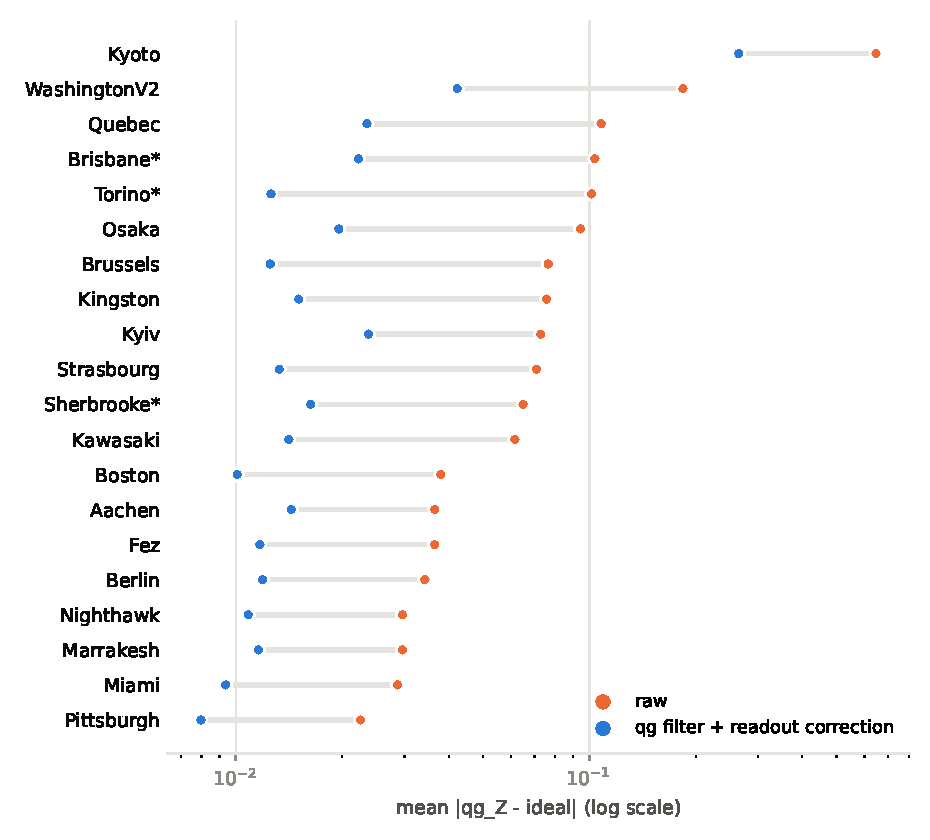
\includegraphics[width=0.78\linewidth]{fig_fleet.pdf}
\caption{Raw and filtered (+ read-out corrected) $\qZ$ error on twenty IBM device noise models. Starred:
§137 (ten circuits, 8000 shots); the others: §144 (five circuits, 4000 shots), devices not used before.}
\label{fig:fleet}
\end{figure}

On the eighteen other fake backends with at least 100 qubits (ECR, CZ and CX devices of 120--156 qubits),
the filter cut the error 2.4--8.9$\times$ on every one of the seventeen that ran (Fig.~\ref{fig:fleet};
median raw / filtered + read-out 3.12). The three predictions nonetheless failed as written: one device
crashed (two predictions required all eighteen), and filter + read-out was lowest on 10 of 17, the filter
alone on the other 7, where read-out errors are small and correcting them adds variance. The crash was a bug
of the library: FakeCusco publishes a qubit that always reads 1, the transpiler placed the circuit on it, and
the read-out inverse was singular. After the fix, \texttt{best\_layout} avoids that qubit and brings the
filtered error from 0.098 to 0.021 (exploratory).

\subsection{Predicting the kept fraction and choosing qubits (§138, §141)}

Over ten layouts per device the prediction ranked the layouts correctly (Spearman 0.94--0.98, passed) and
\texttt{best\_chain} kept 6--17 points more shots than Qiskit's default (passed), but the raw prediction was
low by 0.08--0.13 (failed): it ignored shots that return to the sector. With the mixed-state floor, added
after scoring, the error is 0.023--0.041. For the ring-coupled QNN, \texttt{best\_chain} scored a different
circuit from the one that ran and kept fewer shots on two devices (§139); \texttt{best\_layout} fixes this:
it was never worse than the default and gained 2.2 points where it chose a different layout (§141, two of
three predictions passed).

\subsection{Shot planning (§143)}

For a target error of 0.02 the planner asked for 3000--3400 shots (0.8--0.9 device seconds); over 30
repetitions the worst qubit's error was 0.021--0.023 (passed). The per-qubit prediction was 1.4--1.6$\times$
too low on average (failed): qubits near a pole ($|\qZ|>0.8$) are underestimated 2.4--3.1$\times$, because
noise pulls their $\qZ$ away from $\pm1$; the plan is set by the worst qubit and still met the target.

\subsection{The QNN (§139--§141)}

\begin{table}[h]
\centering\small
\begin{tabular}{lccc}
\toprule
 & raw & filter & filter + read-out\\
\midrule
\texttt{run\_qnn}, default layout (§139) & 545 & 550 & 549\\
\texttt{run\_qnn}, \texttt{best\_chain} (§139) & 547 & 551 & 551\\
\texttt{run\_qnn}, \texttt{best\_layout} (§141) & 545 & 549 & 550\\
qiskit-machine-learning \texttt{SamplerQNN} (§140) & 547 & 548 & --\\
\bottomrule
\end{tabular}
\caption{Correct decisions of 567 (189 inputs on each of three devices; 555 noiselessly), 1000 shots.}
\label{tab:qnn}
\end{table}

The one-job template agrees with per-input circuits (550 against 551, passed) and qiskit-machine-learning
reproduces the library's own path (548, passed), but the filter recovers only 5--6 of the 10 decisions noise
costs, and read-out correction changes no decision (Table~\ref{tab:qnn}). Runs with the identical layout
differ by up to two decisions, so differences of that size are shot noise. Wrapping the QNN in
qiskit-machine-learning 0.9.1 exposed that, with a device pass manager, \texttt{SamplerQNN} reads measured
bits at the physical-qubit positions of the layout, so a circuit measured before transpilation reads every
shot as 0 unless its layout is $[0,\dots,n-1]$; the library transpiles itself and drops the layout, and the
issue was reported upstream.

\subsection{A PCA spectrum (§146)}

Five features, 16 samples from a Gaussian with standard deviations $(2.0,1.4,1.0,0.6,0.35)$ on random axes;
exact spectrum $(0.640,0.203,0.122,0.023,0.011)$; one circuit per sample (4 + 10 RBS, 26--28 native
two-qubit gates), 2000 shots, on the three devices of §137 and the eighteen of §144, FakeCusco included
after the fix. Error is $L_1=\sum_k|\hat\lambda_k-\lambda_k/\sum\lambda|$. All four predictions passed:
noiselessly $L_1=0.020$; all twenty-one ran and filter + read-out was below raw on every one; the median
ratio raw / filter + read-out was 4.6 (1.6--7.7); and the five eigenvalues came out in order on 18 of 21
(raw 13, read-out 14, filter 18). Median $L_1$: raw 0.266, read-out 0.166, filter 0.062, filter + read-out
0.048. The raw estimate is biased upwards for every eigenvalue, because shots that leave the sector add
excitations on all qubits (the raw spectrum sums to more than 1); the filter removes that bias. What
remains is a flattening of the spectrum that grows as the kept share falls: on FakeKyoto (15\% kept) the
order is lost, and on FakeBrisbane only the two smallest eigenvalues, 0.012 apart, swap. Quantum PCA's
exponential speed-up rests on the assumption that copies of $\rho$ are given~\cite{tang2021qpca}; this
experiment makes no claim on it.

\subsection{Hamiltonian simulation and a quantum walk (§147)}

\begin{figure}[h]
\centering
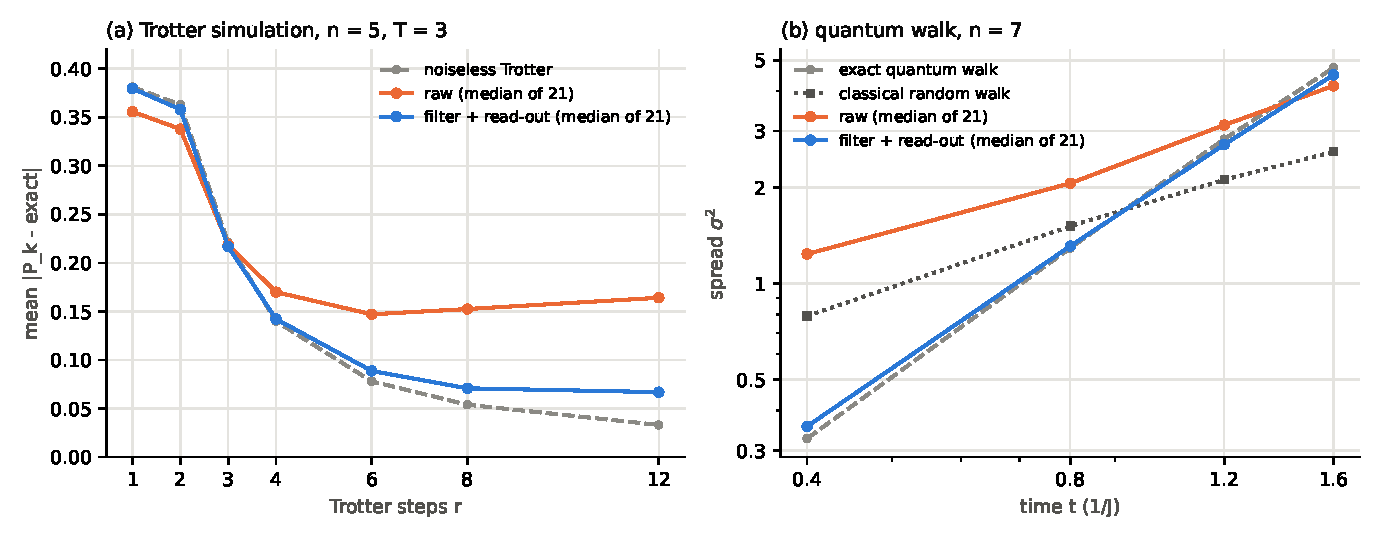
\includegraphics[width=\linewidth]{fig_trotter.pdf}
\caption{(a) Error of the simulated occupations at $T=3$ against the number of Trotter steps (five qubits,
random fields): more steps lower the Trotter error (dashed) and add noise; the filter keeps the error falling
to deeper circuits. (b) Spread of a quantum walk on seven qubits: raw data follow a classical random walk;
filtered data follow the exact quantum walk. Medians over twenty-one device noise models, 4000 shots.}
\label{fig:trotter}
\end{figure}

Part A: $n=5$, $J=1$, $h_k$ uniform in $[-1,1]$, $T=3$, $r\in\{1,2,3,4,6,8,12\}$ (up to 96 native two-qubit
gates). Without noise the Trotter error falls from 0.38 to 0.033; on a device it has a minimum at some $r^*$.
All three predictions passed (Figure~\ref{fig:trotter}a): with filter + read-out the best error is lower than
the best raw error on all twenty-one devices (1.6--2.8$\times$, median 2.0$\times$), $r^*$ is never smaller,
and it is larger on 16 of 21 (median 12 against 8). On eleven devices $r^*=12$, the deepest tested, so the
shift is a lower bound. Part B: $h=0$, $n=7$, the walker on the middle qubit, $t\in\{0.4,0.8,1.2,1.6\}$ with
Trotter step 0.2; the exact spread grows with exponent 1.94, a classical random walk with the same rate with
0.85. Raw data give a median exponent of 0.87: noise spreads the walker from the start and the walk looks
classical (Figure~\ref{fig:trotter}b). With filter + read-out the median exponent is 1.84, the raw exponent is
lower on 20 of 21 (passed), and $\sigma^2$ is within 20\% of the exact value at all four times on 15 of 21
(raw: none; passed). The exponent reached 1.5 on 16 devices, not the predicted 18 (failed): the four noisiest
after FakeKyoto give 1.26--1.38, and on FakeKyoto (15\% of shots kept at 96 gates) the walk is lost.

\subsection{Interacting excitations (§148)}

\begin{table}[h]
\centering\small
\begin{tabular}{lccccc}
\toprule
excitations & raw & read-out & filter & filter + read-out & raw / filter + read-out\\
\midrule
1 & 0.066 & 0.038 & 0.008 & 0.009 & 5.6 (2.4--14.4)\\
2 & 0.080 & 0.072 & 0.030 & 0.028 & 2.6 (1.1--3.8)\\
3 & 0.065 & 0.055 & 0.030 & 0.024 & 2.6 (1.0--4.6)\\
\bottomrule
\end{tabular}
\caption{XXZ chain, $n=6$, $V=2$, $T=2$: best error over Trotter order (1, 2) and steps (1--8), median over
twenty-one device noise models; the last column is the median ratio and its range across devices.}
\label{tab:xxz}
\end{table}

One excitation is the filter's easiest case and is easy classically too. With $V=2$, random fields in
$[-0.5,0.5]$, $T=2$ and 1, 2 or 3 excitations starting on the first qubits of a six-qubit chain, the dynamics
is many-body. The filter's benefit falls from 5.6$\times$ with one excitation to 2.6$\times$ with two and with
three (Table~\ref{tab:xxz}; predicted to fall with each excitation, passed only just between two and three).
Sectors with more excitations keep more shots (0.49 against 0.43 at 120 two-qubit gates) yet gain less: more
of the noise lands inside a larger sector (20 of 64 states at half filling, against 6), where the filter
cannot see it. Filter + read-out was best on 62 of the 63 device--sector pairs; on FakeKyoto at half filling
it was not (0.238 against 0.231), so that prediction failed. The filter again moved the optimal number of
Trotter steps deeper (61 of 63; median 8 or 6 against 4), and second-order Trotter was better with two
excitations on 20 of 21 devices (passed); with three, only on 5, because its extra gates cost more than its
smaller Trotter error saves. Building this experiment showed that the transpiler pass read state-preparation
X gates in the order the DAG lists them and could misreport the initial weight; it now takes an X as
preparation when it is the first operation on its qubit.

\section{Discussion}

As a read-out tool the filter is robust: on every one of twenty IBM device noise models it lowered the $\qZ$
error by a factor of 2.4 or more, and it combines with read-out correction and with zero-noise extrapolation.
Which combination is best depends on the device: read-out correction helps where read-out errors are large
and adds variance where they are small. The calibration also tells, before any device time is spent, how many
shots the filter will keep, which qubits keep most, and how many shots a target precision needs.

The limits are as clear. The gain in classification accuracy is small, because the model's decisions are
mostly far from threshold; spectrum estimation, where the answer is a set of
probabilities rather than a decision, gains more (4.6$\times$), and so does
dynamics: the filter lets a Trotter simulation use more steps and makes the ballistic spreading of a quantum
walk visible where raw data look classical. Its benefit is largest with one excitation and halves when the
excitations interact. Eleven of the thirty-seven predictions failed as written, several through the analysis rather
than the filter: a prediction that ignored returning shots, a per-qubit error model that ignored the poles,
and an experiment that required every device to run. And all results are on device noise models, which
model gate, relaxation, dephasing and read-out errors as independent channels; leakage, crosstalk and drift
are absent. A run on hardware is the next step.

\section*{Code and data availability}

Everything is in the open-source library qang (MIT license), version 0.10.0 and later:
\url{https://github.com/Viny2030/qang}, \texttt{pip install qang}. The module is \texttt{qang.ibm} (with
\texttt{qang.qiskit\_ml}); each section has a script in \texttt{examples/} and its output in
\texttt{examples/data/}; \texttt{docs/ibm\_quickstart.md} shows the workflow.

\begin{lstlisting}[language=Python]
from qang import ibm
t = transpile(qc, backend)                 # qc: weight-preserving, measured
res = Sampler(mode=backend).run([t]).result()[0]
ibm.ibm_qg(res, t, backend, weight=1)["filtered_readout"]
\end{lstlisting}

\bibliographystyle{unsrtnat}
\bibliography{../refs}

\end{document}
